\chapter{Снижение размерности динамической модели нефтегазового месторождения}\label{ch:ch2}

\todo{7 pages}

\todo{TODO nomenclature}

\newcommand{\bvec}[1]{\mathbf{#1}}
\newcommand{\resid}{\bvec{r}}
\newcommand{\unk}{\bvec{u}}
\newcommand{\jac}{\mathrm{J}}
\newcommand{\dunk}{\Delta \unk}
\newcommand{\vunk}{\bvec{v}}
\newcommand{\matr}[1]{\mathrm{\uppercase{#1}}}
\newcommand{\norm}[2][~]{\left\| #2  \right\|_{#1}}
\newcommand{\transpose}[1]{\matr{#1}^\mathrm{T}}
\newcommand{\dvunk}{\Delta \vunk}
\newcommand{\deriv}[3][]{\frac{\partial^{#1} #2}{\partial #3^{#1}}}
\newcommand{\pc}[1][~]{\bvec{\varphi}_{#1}}
\newcommand{\param}{\bvec{\mu}}
\newcommand{\nlin}{\bvec{\eta}}

\todo{TODO dimensionality of vectors}

\section{Определяющие уравнения}

\subsection{Модельная задача}

\begin{figure}[ht]
    \centerfloat{
        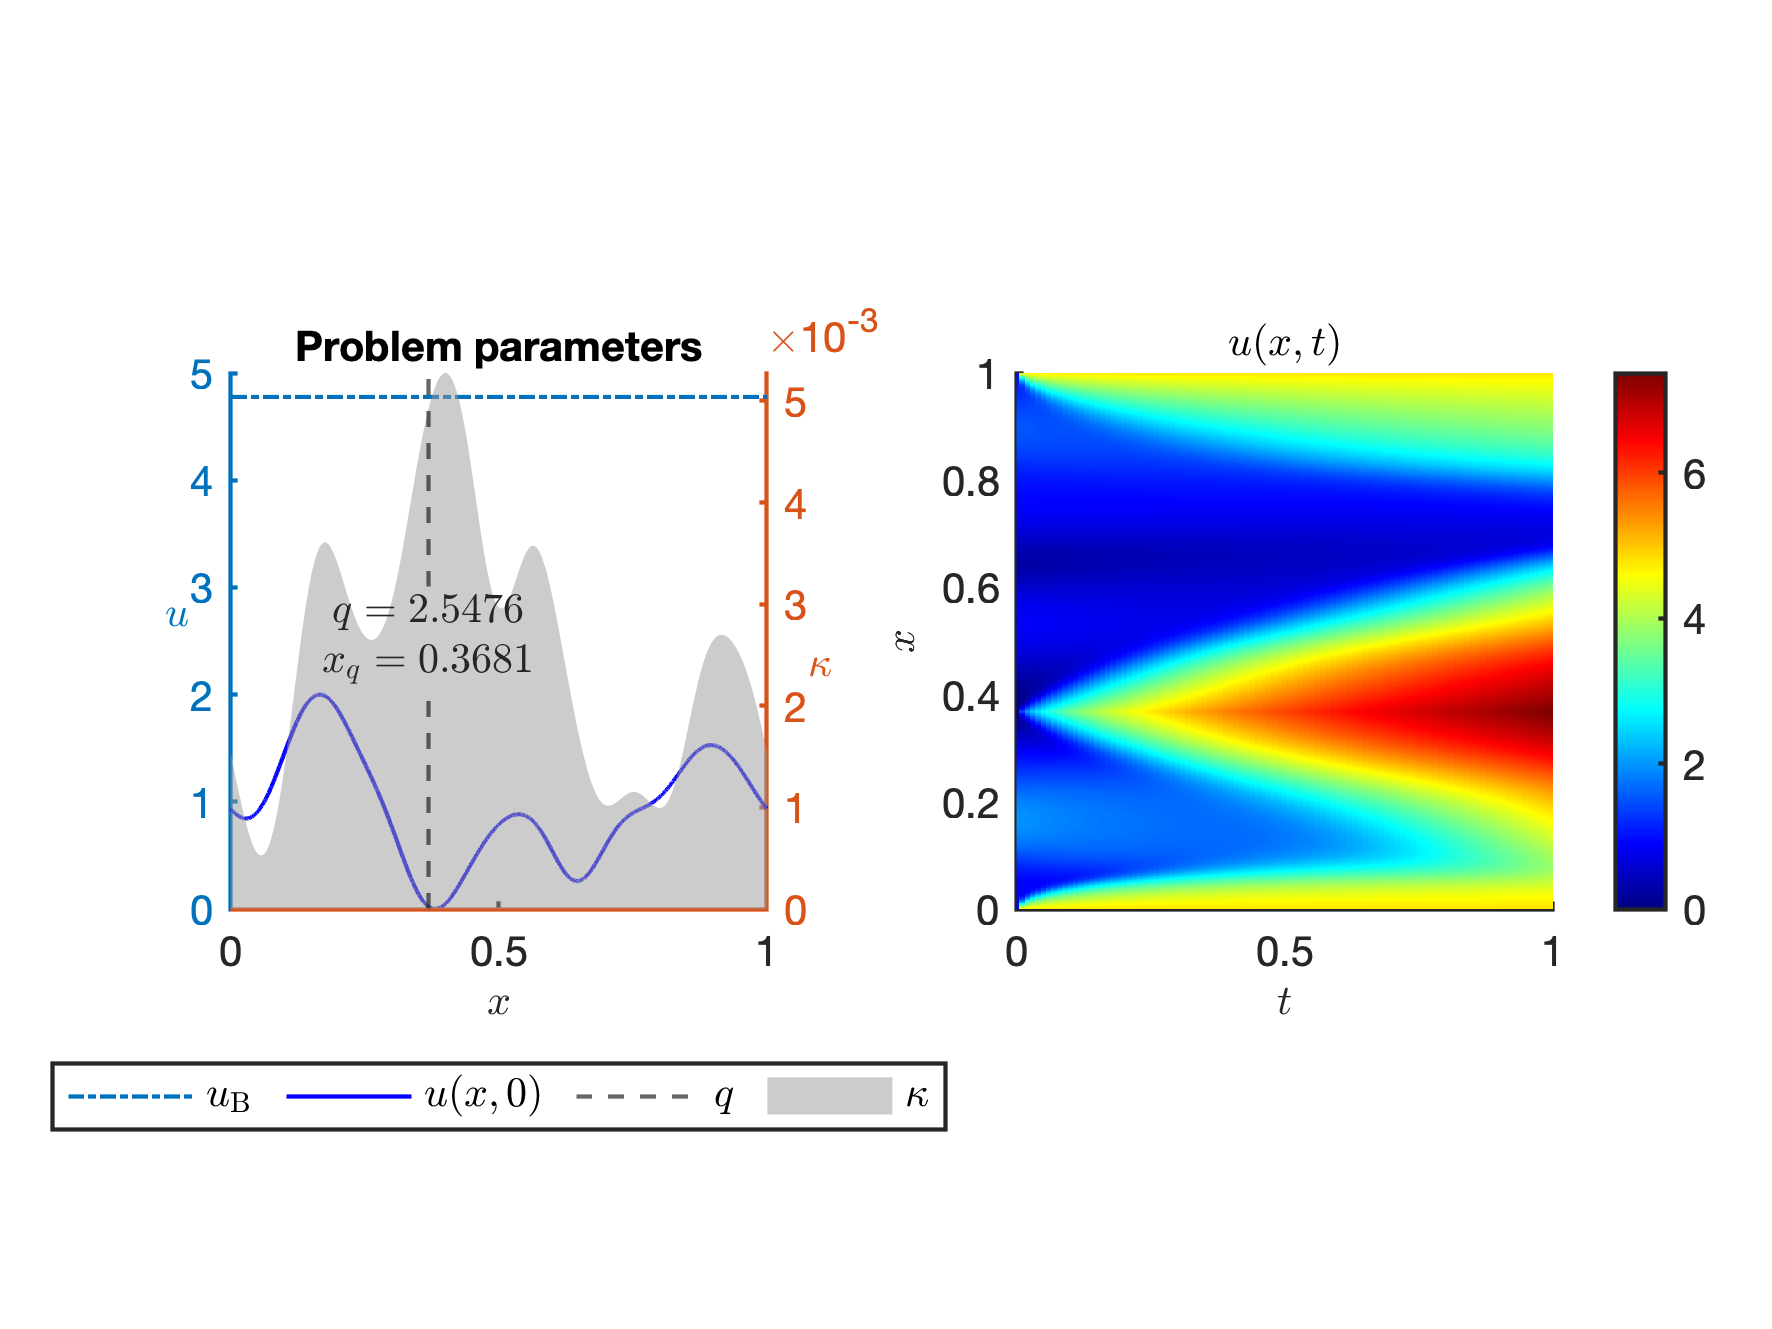
\includegraphics[width=\textwidth,trim={0 1.5cm 0 2.5cm},clip]{./sci_report/images/ECMOR/1-FOM.png}
    }
    \caption{\todo{caption}}\label{fig:FOM}
\end{figure}

\subsection{\todo{Система уравнений чёрной нефти}}

\begin{multline}
    \deriv{~}{t}\left(
        \varphi \matr{R}_{\alpha A} \frac{s_A}{b_A}
    \right) - \overrightarrow{\nabla} \left[
        \matr{R}_{\alpha A} \left(
            K\frac{\varkappa_A}{\mu_A b_A}\nabla p
        \right)
    \right] \\
    = \matr{R}_{\alpha A}
    \frac{2\pi K \varkappa_A}{\mu_A b_A \ln(r_c r_\text{well}^{-1})}
    \left(p - p_\text{well}\right)
\end{multline}

\begin{align}
    \sum_A s_A = 1
\end{align}

\section{Методы анализа данных для снижения размерности и предобуславливания}

\subsection{Снижение размерности нелинейной модели}

\begin{equation}
   \resid(\unk) = 0
\end{equation}

\begin{equation}
    \unk_\ast = \arg \min_{\unk} \norm{\resid(\unk)}
\end{equation}

\begin{equation}
    \resid(\unk + \Delta \unk) \approx \resid(\unk) + \jac(\unk) \dunk
\end{equation}

\begin{align}
    \dunk_\ast (\unk) = \arg \min_{\dunk} \norm[2]{\resid(\unk) + \jac(\unk) \dunk} \\
    \jac = \deriv{\resid}{\unk} \\
    \jac(\unk) \dunk_\ast = - \resid(\unk)
\end{align}

\begin{align}
    \unk_\Phi (\vunk) = \Phi \vunk \\
    \dim{\vunk} \leq \dim{\unk} \\
    \norm{\unk_\Phi - \unk} \\
    \Phi^{-1} = \transpose{\Phi}
\end{align}

\begin{align}
    \dvunk_\ast = \arg \min_{\dvunk} \norm[2]{\resid(\Phi \vunk) + \jac(\Phi \vunk) \Phi \dvunk} \\
    \transpose{P}\jac \dvunk_\ast = - \transpose{P} \resid
\end{align}

\begin{align}
    \matr{P}_\text{G} = \Phi \\
    \matr{P}_\text{LS} = \jac \Phi \\
    \Delta x \rightarrow 0
\end{align}

\begin{align}
    \norm{\resid(\Phi \vunk_\ast)} \\
    \norm{\transpose{P}\resid(\Phi \vunk_\ast)}
\end{align}

\begin{equation}
    \varepsilon_\text{FOM} = \norm{\frac{\resid}{\dim{\resid}}} \leq \varepsilon \\
\end{equation}

\begin{equation}
    \varepsilon_\text{ROM} = \norm{\frac{\transpose{\matr{P}_\text{G}}\resid}{\dim{ \transpose{\matr{P}_\text{G}}\resid}}} \leq \varepsilon
\end{equation}

\subsection{Правильное ортогональное разложение}

\begin{align}
    \unk_0 \\
    \unk_n = \arg \min_{\unk} \norm{\resid(\unk,\unk_{n-1};\param)}
\end{align}

\begin{align}
    \unk_\text{o} (= \unk_0 (= 0 ?)) \\
    \matr{U} (\param) =
    \begin{bmatrix}
        \unk_0, \unk_1, \dots, \unk_{N_t}
    \end{bmatrix}
\end{align}

\begin{align}
    \matr{u} - \unk_\text{o} = \Phi \Sigma \transpose{\Upsilon} \\
    \Phi^{-1} = \transpose{\Phi} \\
    \Phi = \begin{bmatrix}
        \widetilde{\Phi}, \pc[N_\vunk + 1], \dots
    \end{bmatrix}
\end{align}

\begin{align}
    \unk_{\widetilde{\Phi}} = \widetilde{\Phi} \vunk \\
    \unk_{\widetilde{\Phi}}(\unk) = \widetilde{\Phi} \transpose{\widetilde{\Phi}} \unk
\end{align}

\begin{figure}[ht]
    \centerfloat{
        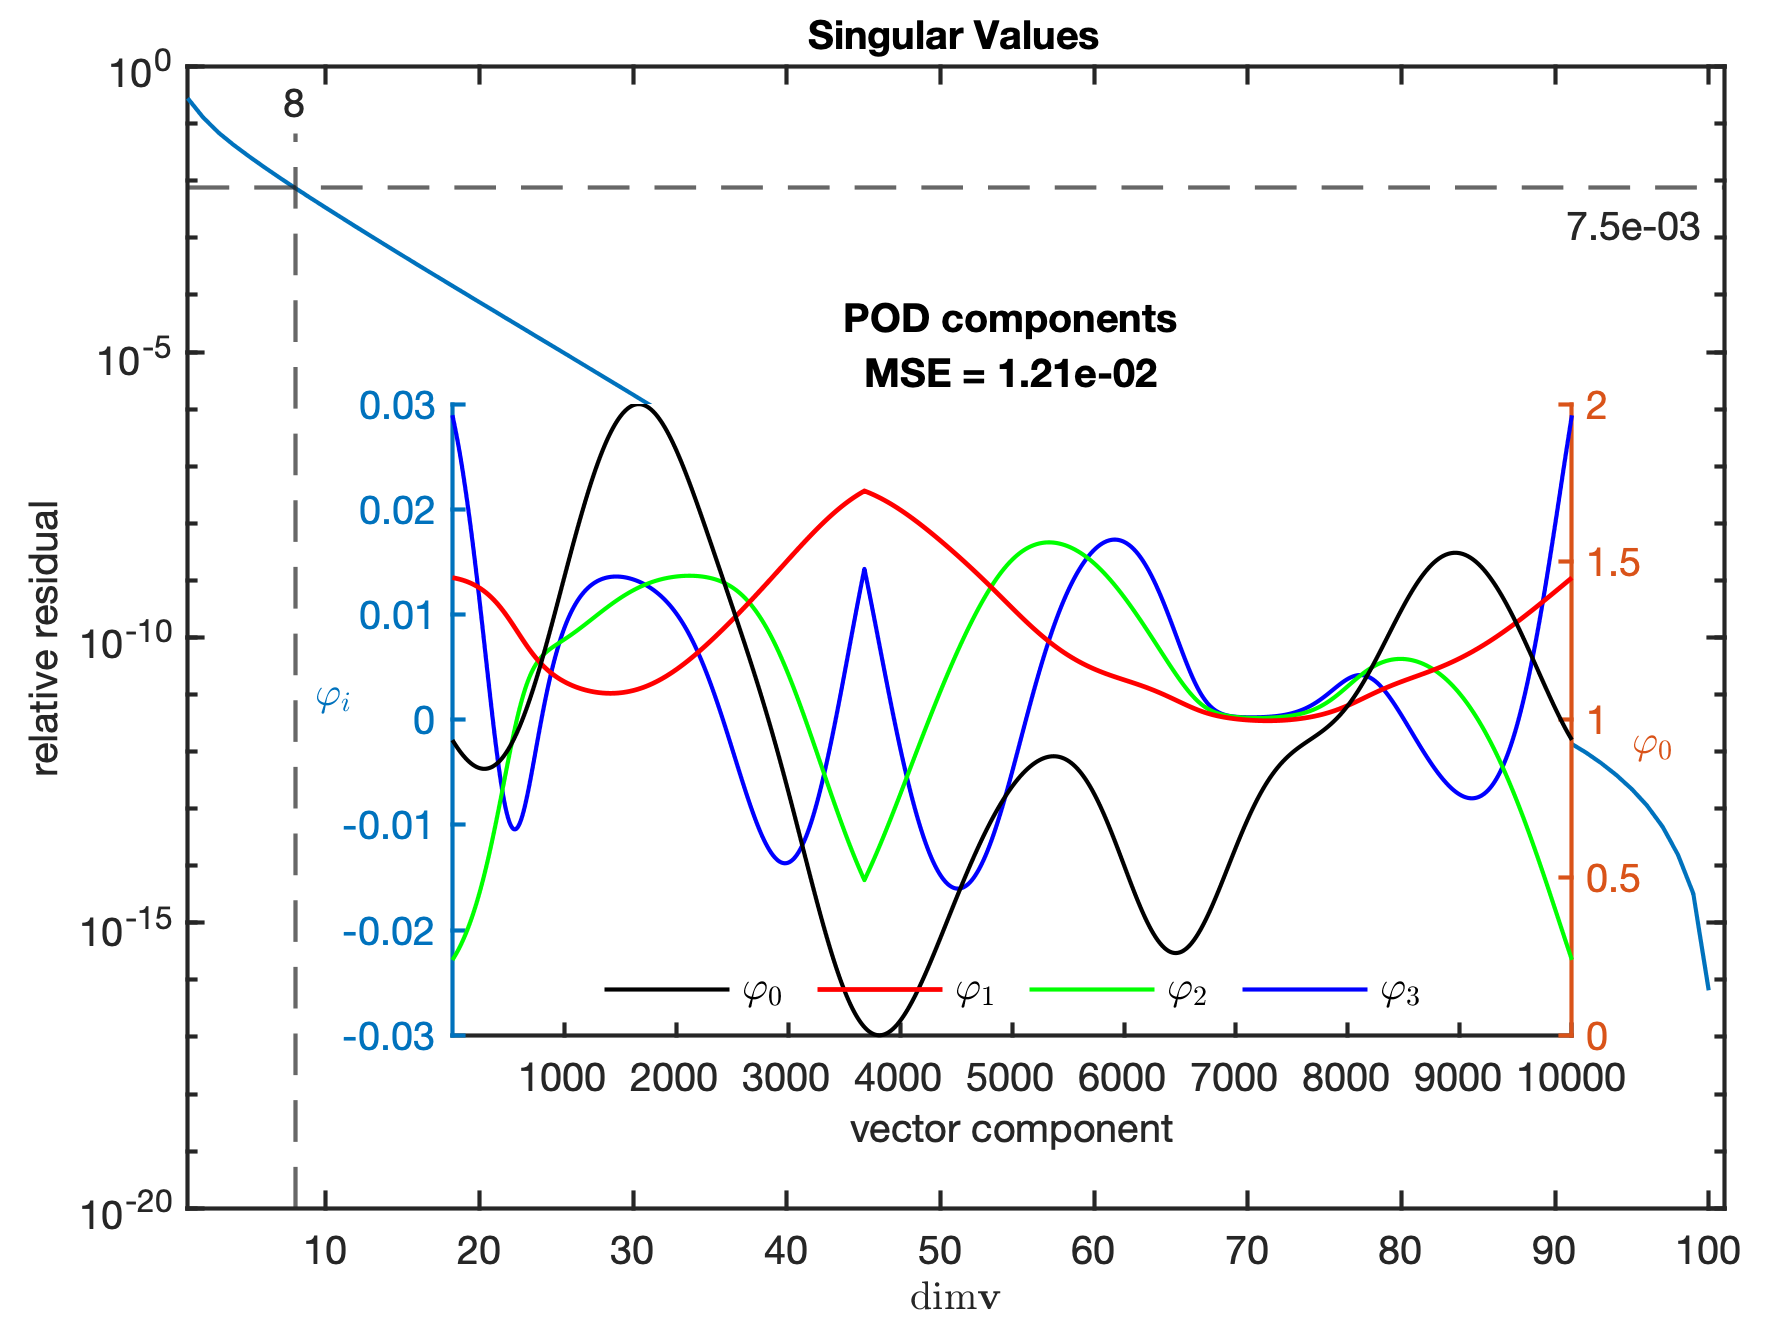
\includegraphics[scale=1]{./sci_report/images/ECMOR/2-POD.png}
    }
    \caption{\todo{caption} \cite{Elizarev2022}}\label{fig:POD}
\end{figure}

\subsection{Выбор главных компонент в триангулированной области параметров}

\begin{figure}[ht]
    \centerfloat{
        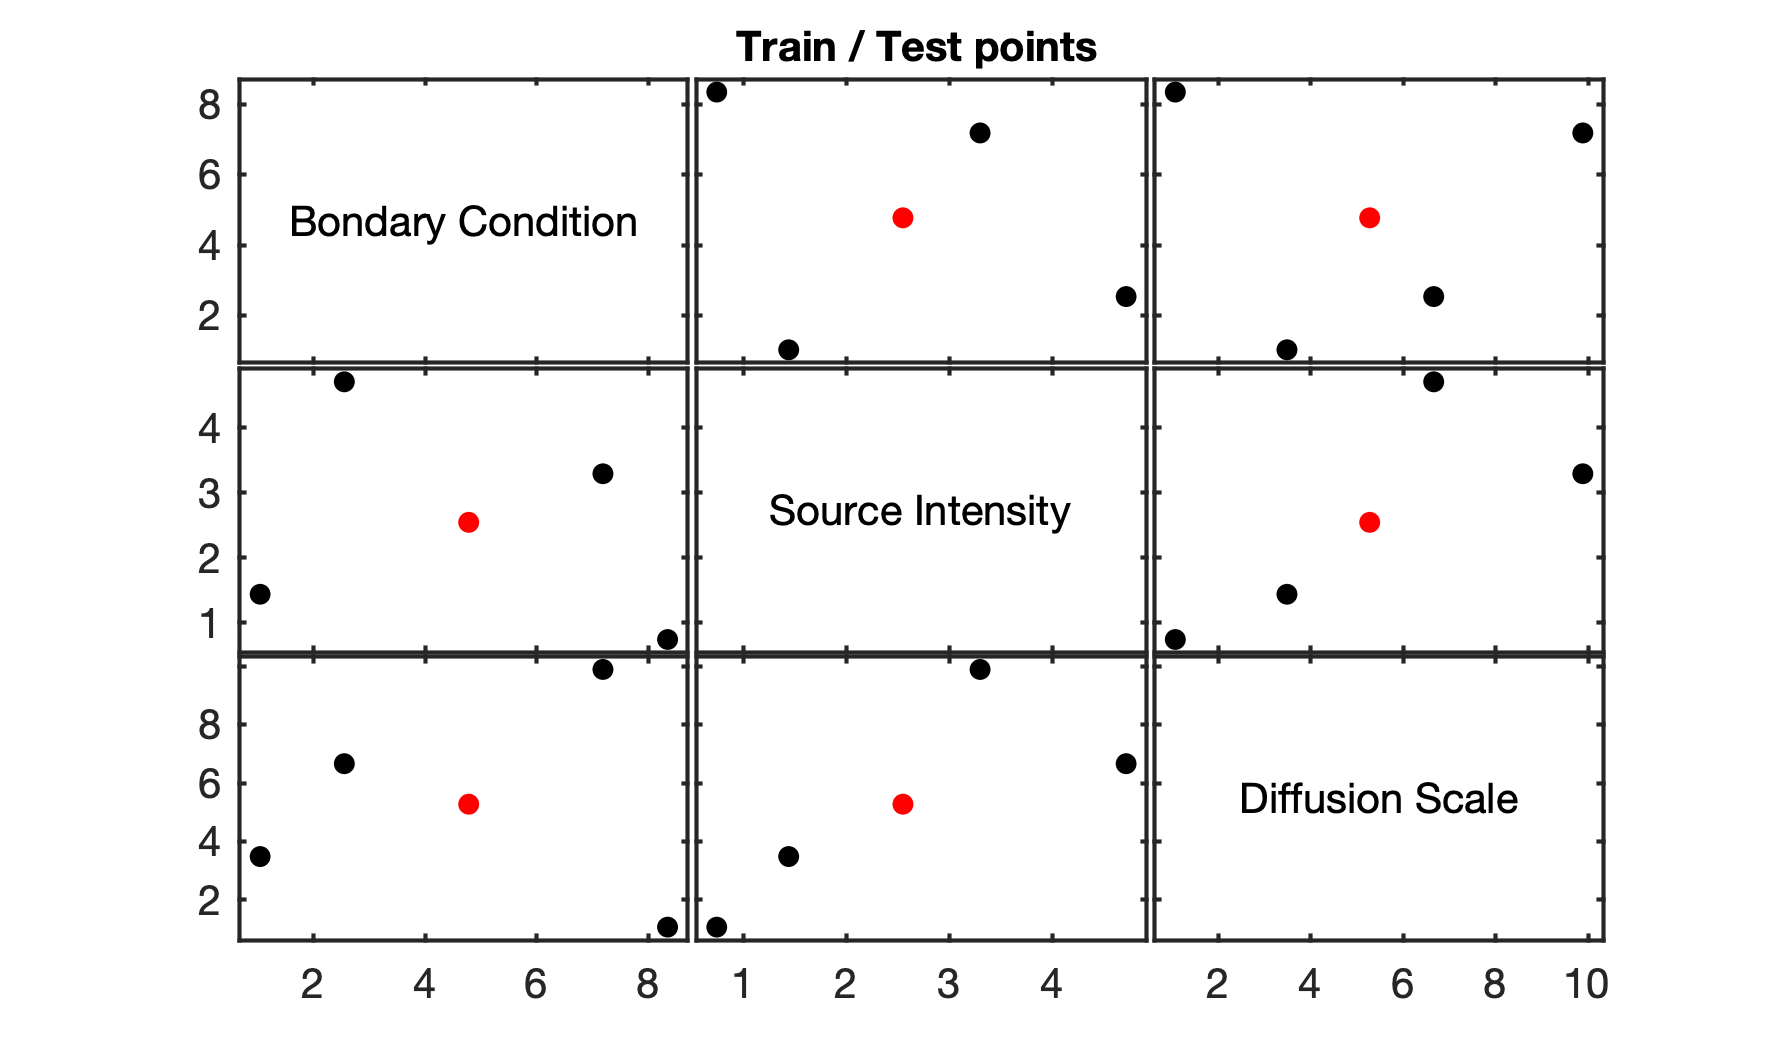
\includegraphics[scale=1]{./sci_report/images/ECMOR/6-Train-Test.png}
    }
    \caption{\todo{caption} \cite{Elizarev2022}}\label{fig:params}
\end{figure}

\begin{align}
    \matr{M} =\begin{bmatrix}
        \param_1, \dots, \param_{N_\param}
    \end{bmatrix}\\
    \matr{U}(\matr{M}) =
    \begin{bmatrix}
        \matr{U}(\param_1), \dots, \matr{U}(\param_{N_\param})
    \end{bmatrix}
    \rightarrow \widetilde{\Phi (\matr{M})} \\
    \widetilde{\Phi} (\matr{M}) \matr{R}_\text{qr} =
    \begin{bmatrix}
        \widetilde{\Phi}(\param_1), \dots,  \widetilde{\Phi}(\param_{N_\param})
    \end{bmatrix}
\end{align}

\begin{equation}
N_\vunk : \widetilde{\Phi} \in \mathbb{R}^{N_\unk \times N_\vunk}
\end{equation}

\begin{figure}[ht]
    \centerfloat{
        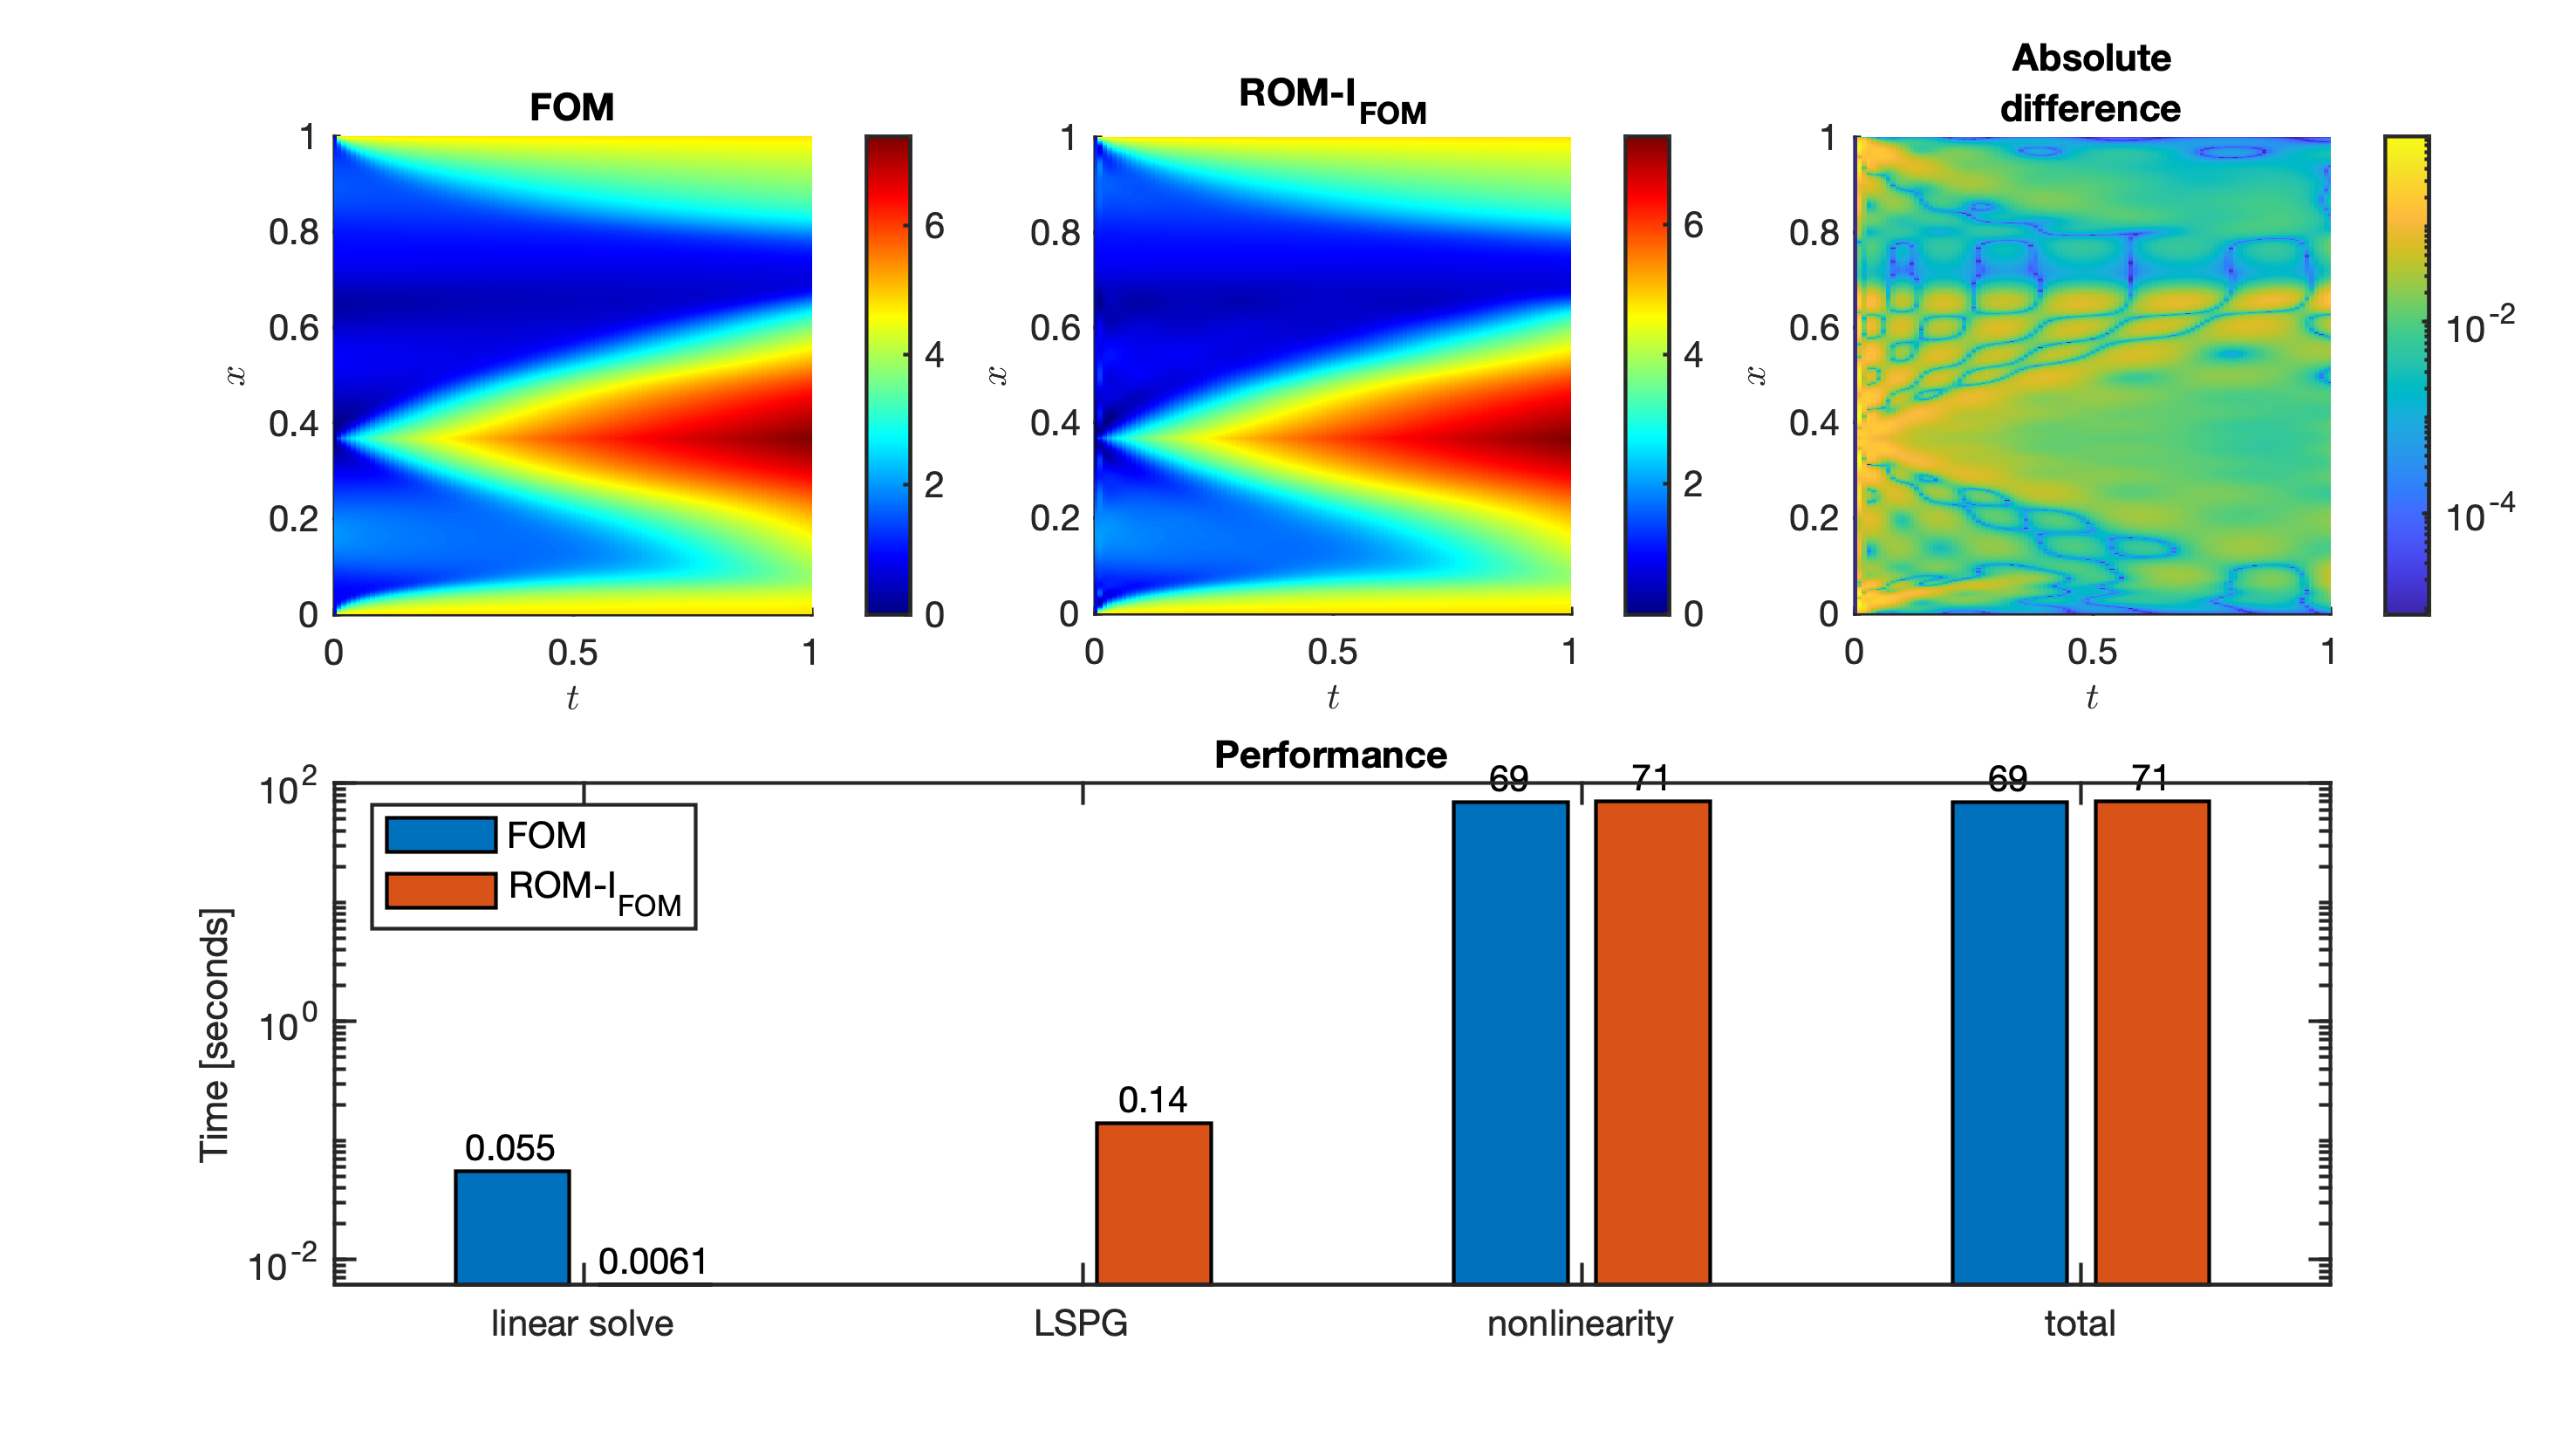
\includegraphics[width=\textwidth]{./sci_report/images/ECMOR/3-ROM-I.png}
    }
    \caption{\todo{caption} \cite{Elizarev2022}}\label{fig:ROM-I}
\end{figure}

\subsection{Аппроксимация нелинейных функций высокой размерности}

\begin{align}
 \nlin(\unk) \rightarrow \nlin (\unk_{\widetilde{\Phi}}) = \nlin (\widetilde{\Phi} \vunk) \\
 \dim{\nlin} \sim \dim{\unk}
\end{align}

\begin{align}
    \mathcal{N} =
    \begin{bmatrix}
        \nlin_1, \dots,  \nlin_{N_\nlin}
    \end{bmatrix} \\
    \mathcal{N} \rightarrow \widetilde{\Phi}_\mathcal{N} \\
    \nlin \approx \widetilde{\Phi}_\mathcal{N} \bvec{\gamma}
\end{align}

\begin{align}
   \bvec{\rho} : \rho_m \in \left\{0, 1 \right\} \\
   N_{\bvec{\rho}} = \sum_m \rho_m \\
   \matr{P} \in \mathbb{R}^{\dim{\nlin} \times N_{\bvec{\rho}}} \\
   \overline{\nlin} = \transpose{P} \nlin
\end{align}

\begin{figure}[ht]
    \centerfloat{
        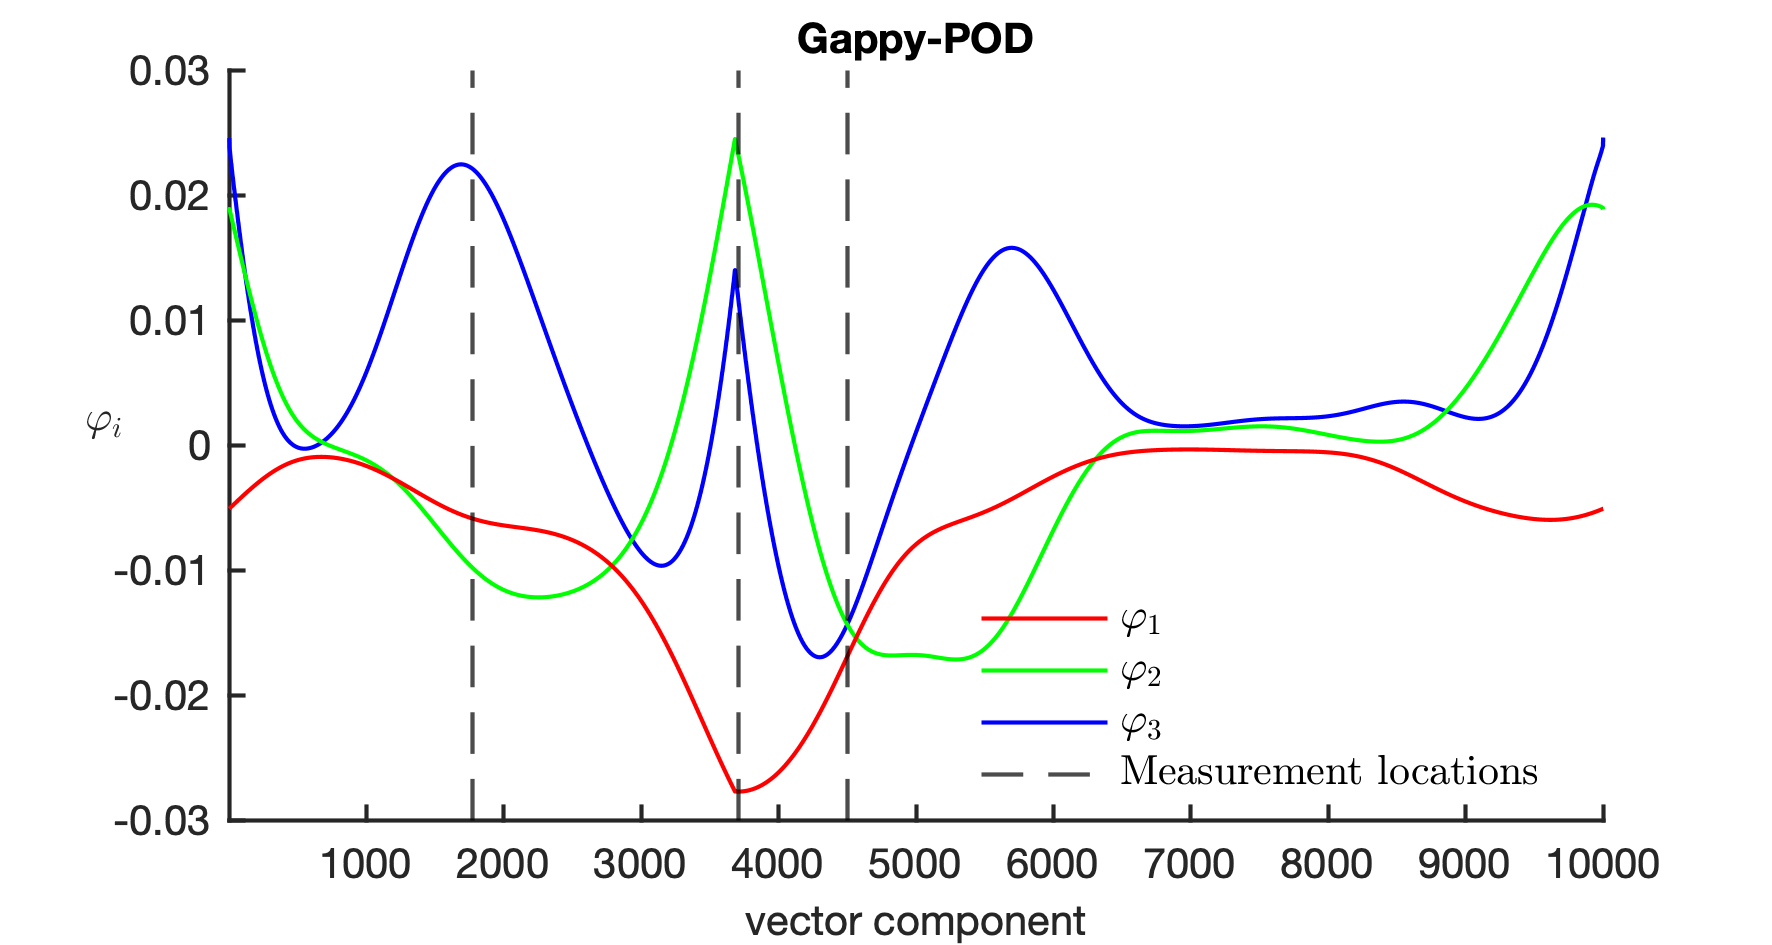
\includegraphics[scale=1]{sci_report/images/ECMOR/4-Gappy.png}
    }
    \caption{\todo{caption}~\cite{Elizarev2022}}\label{fig:gappy}
\end{figure}

\begin{align}
    \widehat{\bvec{\gamma}} = \arg \min_{\bvec{\gamma}} \norm[2]{\transpose{P} \widetilde{\Phi}_\mathcal{N} \bvec{\gamma} - \overline{\nlin}} \\
    \widehat{\bvec{\gamma}} = {\left( \transpose{P} \widetilde{\Phi}_\mathcal{N} \right)}^\dagger \overline{\nlin} = \mathcal{O} \overline{\nlin} \\
    \widehat{\nlin} = \widetilde{\Phi}_\mathcal{N} \widehat{\bvec{\gamma}} = \matr{\Pi} \overline{\nlin}
\end{align}


\begin{align}
    \dvunk_\ast (\vunk)= \arg \min_{\dvunk} \norm[2]{\widehat{\resid}(\Phi \vunk) + \widehat{\jac}(\Phi \vunk) \Phi \dvunk}
\end{align}

\begin{align}
    \matr{\matr{L}} \nlin \approx
    \matr{\matr{L}} \matr{\Pi} \overline{\nlin} = \widehat{\matr{\matr{L}}} \overline{\nlin}
\end{align}

\begin{figure}[ht]
    \centerfloat{
        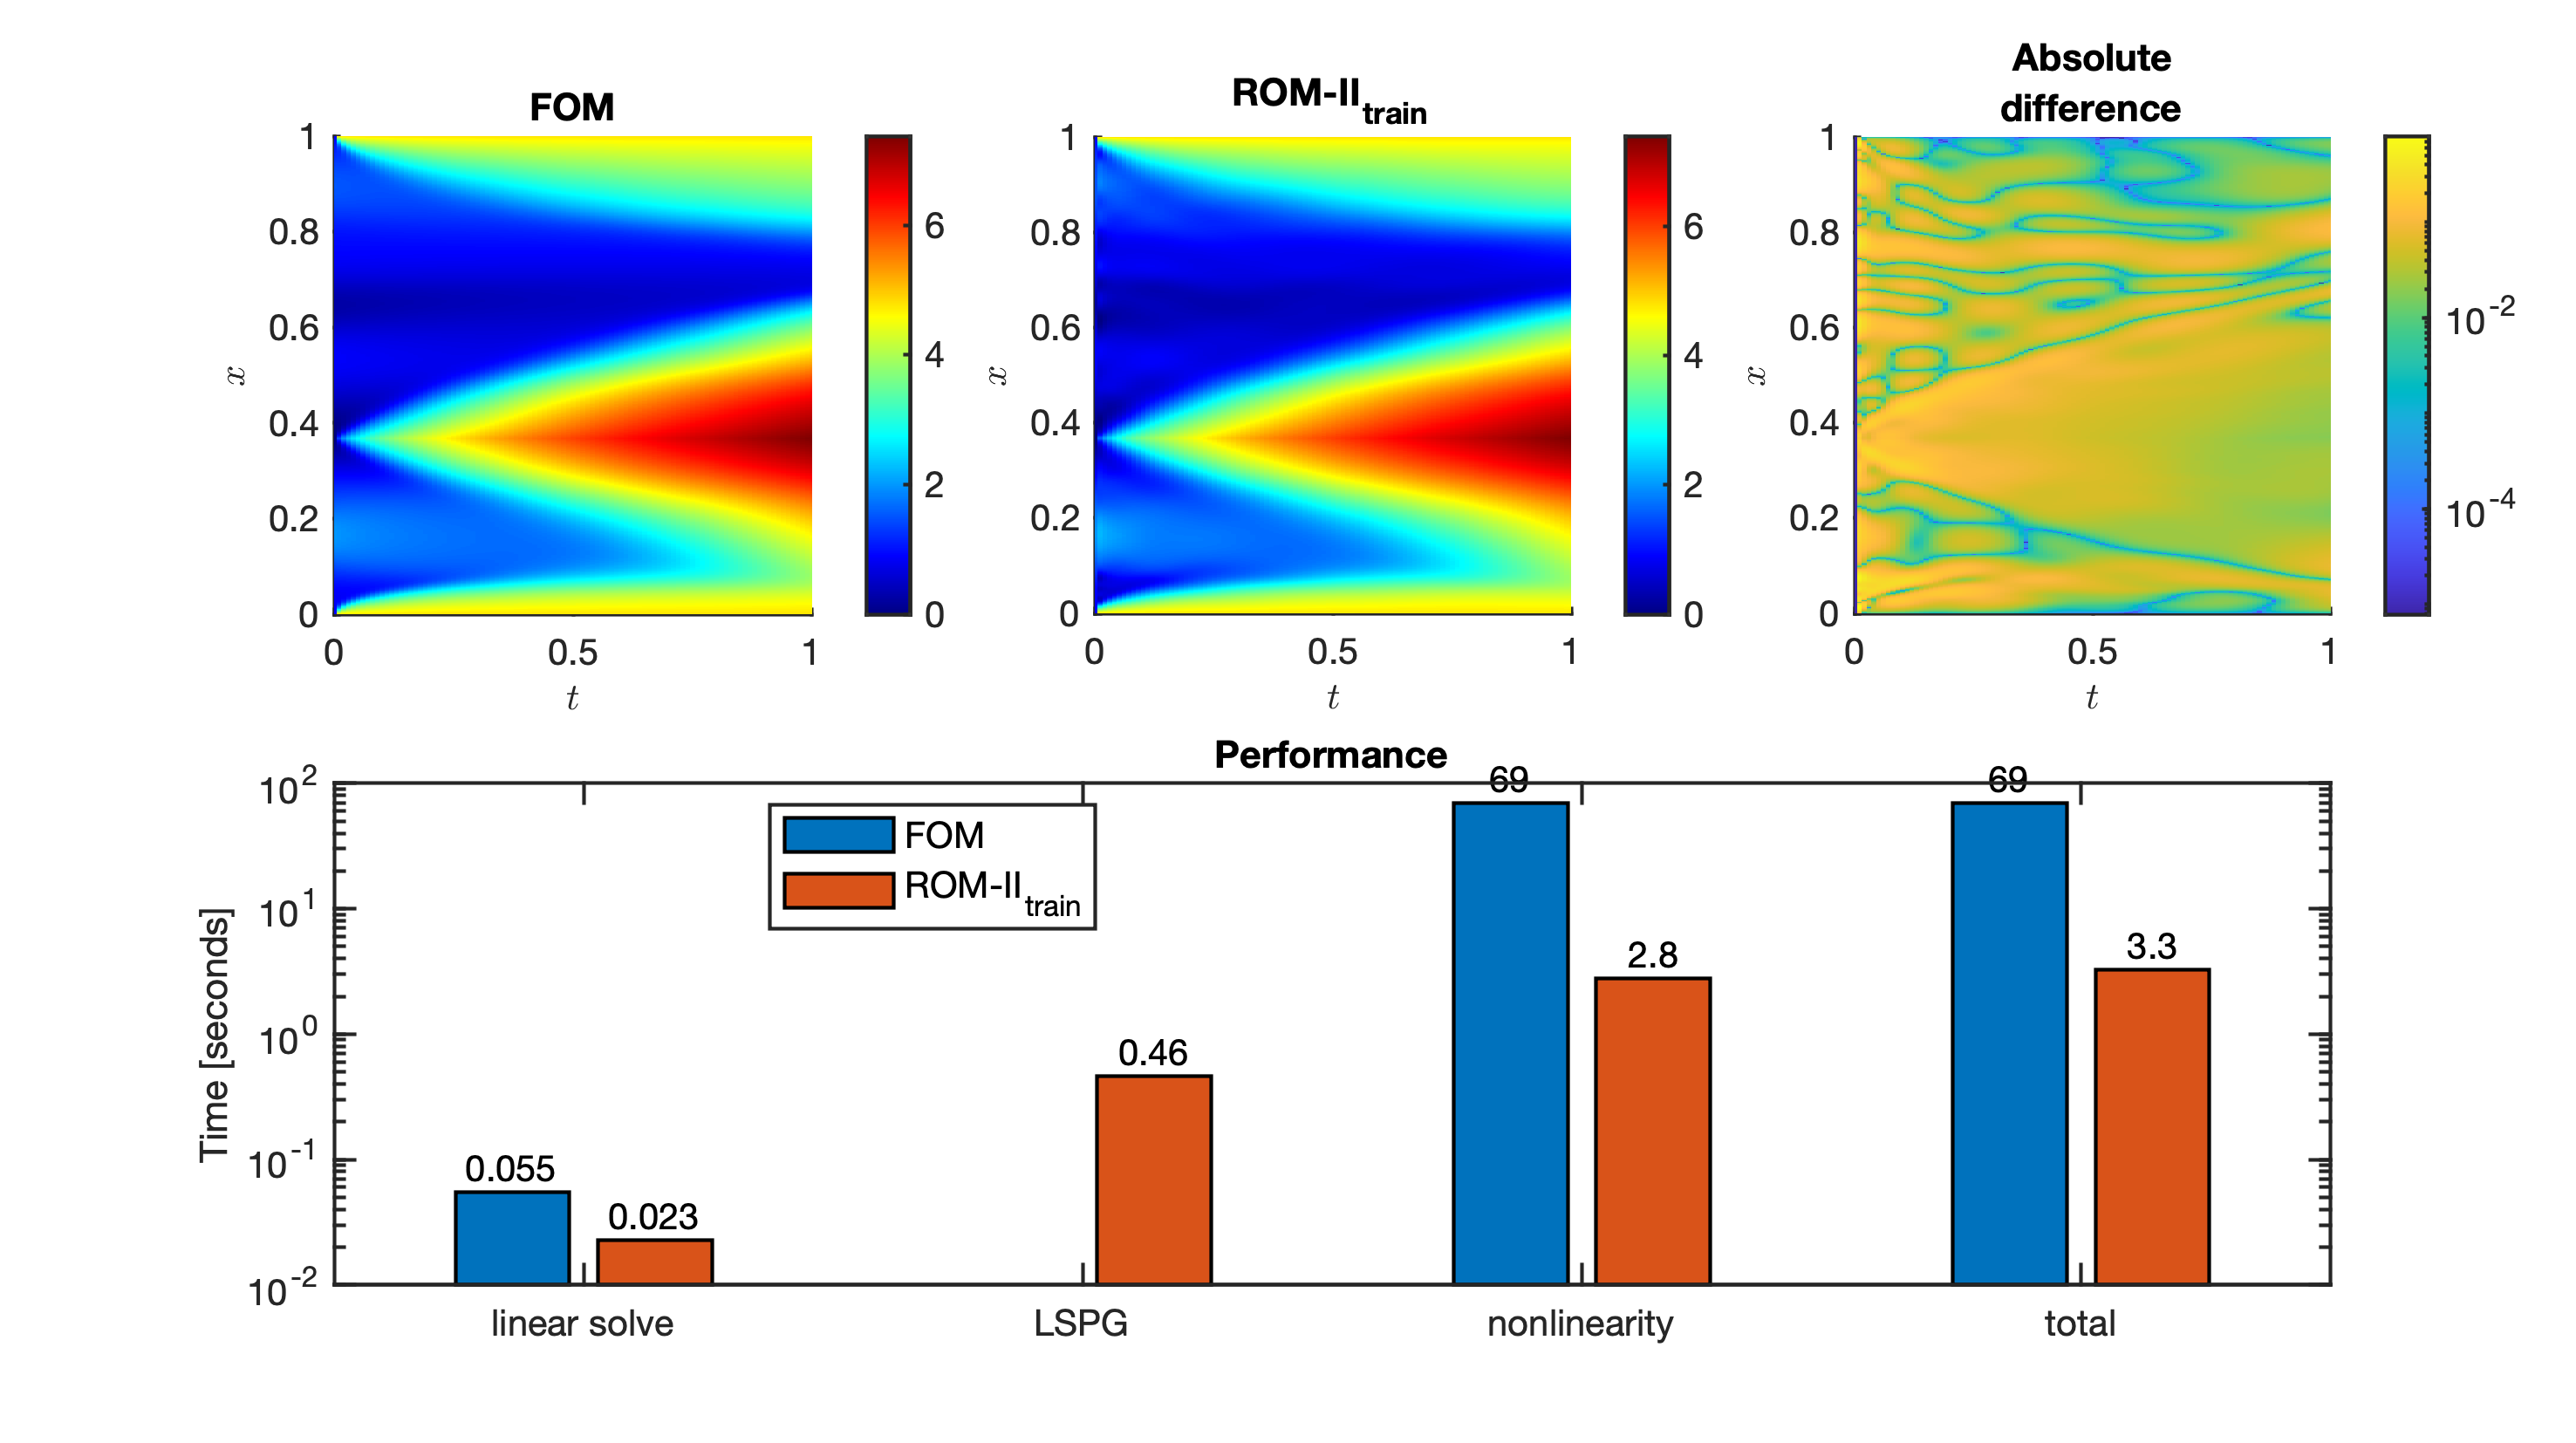
\includegraphics[width=\textwidth]{./sci_report/images/ECMOR/7-ROM-II-Train.png}
    }
    \caption{\todo{caption} \cite{Elizarev2022}}\label{fig:ROM-II}
\end{figure}

\subsection{Использование данных для предобуславливания}

\begin{equation}
    \unk_{n+1} \approx \matr{D} \unk_{n}
\end{equation}

\begin{align}
    \matr{U}_{-} &=
    \begin{bmatrix}
        \unk_0, \dots, \unk_{N_t-1}
    \end{bmatrix}\\
    \matr{U}_{+} &=
    \begin{bmatrix}
        \unk_1, \dots, \unk_{N_t}
    \end{bmatrix}
\end{align}

\begin{align}
    \matr{D} = \arg \min_{\matr{A}} \norm[\text{fro}]{\matr{U}_{+} - \matr{D} \matr{U}_{-}} = \matr{U}_{+} \matr{U}_{-}^{\dagger}
\end{align}

\begin{align}
    \widetilde{\Phi} \vunk_{n+1} \approx  \matr{D} \widetilde{\Phi} \vunk_{n} \\
    \vunk_{n+1} \approx  \matr{D}_{\widetilde{\Phi}} \vunk_{n} \\
\end{align}

\begin{align}
    \left\{ \Psi_{\widetilde{\Phi}},  \widetilde{\Lambda} \right\} : \matr{D}_{\widetilde{\Phi}}  \Psi_{\widetilde{\Phi}} = \Psi_{\widetilde{\Phi}} \widetilde{\Lambda} \\
    \widetilde{\Psi} = \widetilde{\Phi} \Psi_{\widetilde{\Phi}} \widetilde{\Lambda} \\
    \matr{D} \widetilde{\Psi} = \widetilde{\Psi}\widetilde{\Lambda} \\
    \left\{\widetilde{\Psi},  \widetilde{\Lambda} \right\} \rightarrow \widetilde{\matr{D}}\\
    \unk_{n+1} \approx \widetilde{\matr{D}} \unk_{n}
\end{align}

\begin{align}
   \unk \rightarrow \nlin(\unk) \rightarrow \matr{D}_{\nlin}
\end{align}

\begin{align}
    \exists \nlin(\unk), \matr{\mathcal{K}} : \nlin_{n+1} \equiv \matr{\mathcal{K}}  \nlin_{n}
 \end{align}

\begin{align}
    \unk_{n+1} \approx \matr{D} \unk_{n} + \matr{B} \bvec{q}_{n} + \matr{C} \bvec{q}_{n+1}
\end{align}

\subsection{\todo{Иерархия эмпирических методов ускоренного моделирования}}

\begin{figure}[ht]
    \centerfloat{
        \includegraphics[width=\textwidth]{./sci_report/images/seminar/ROM-ROM-3.png}
    }
    \caption{\todo{caption} \cite{Elizarev2022}}\label{fig:ROM-II}
\end{figure}

\subsubsection{\todo{Накопление данных в итеративных прямых расчётах}}

multi-level Monte Carlo
